\documentclass[11pt]{article}
\usepackage{amsmath, amssymb, amsfonts}
\usepackage[margin=1in]{geometry}
\usepackage{fancyhdr}
\usepackage{tcolorbox}
\usepackage{enumerate}
\usepackage{tikz}
\usepackage{subcaption}

\usepackage{algorithmic}

\newcommand{\zo}{\{0,1\}}


\begin{document}

    \setlength{\headheight}{26pt}
    \pagestyle{fancy}
    \fancyhead[C]{\textbf{Basic Algorithms (Section 5)}\\Spring 2025}
    \fancyhead[R]{HW3 (Due 2/20 23:59)\\ Instructor: Jiaxin Guan}
    \fancyfoot[C]{}
    \fancyfoot[R]{\thepage}
    \renewcommand{\headrulewidth}{0.4pt}
    \renewcommand{\footrulewidth}{0.4 pt}
    
    %%%% EDIT THIS PART 
    %Put your name and Net ID here
    \fancyhead[L]{Name: Nick Zhu \\ Net ID: xz4687}
    %Write your collaborators' names here
    \fancyfoot[L]{Discussion Partners:}
    %%%%%
	
    
    %Problem 1
    \begin{tcolorbox}[title={Problem 1 (Divide and Conquer the Peak, 30 pts)}]
        Suppose we have an array $A$ of $n$ distinct integers and moreover are guaranteed that the array has the following property: up to some index $1\leq i \leq n$, $A$ is increasing, i.e., $A[1] < A[2] < \ldots < A[i]$, and then after index $i$, $A$ is decreasing, i.e., $A[i] > A[i+1] > \ldots > A[n]$. In this array, we call $A[i]$ the \emph{peak} of $A$. For example, consider the array $[1, 4, 7, 8, 6, 2]$, which has peak $8$. 
        \medskip
        
        Create an algorithm that finds the peak of an input array $A$ in sublinear time (i.e. $o(n)$). Justify the correctness and time complexity of your proposed algorithm.
    \end{tcolorbox}
    %Write your solution here!
    \section*{Solution}
    The key observation is that since the array is first increasing and then decreasing, a binary search can be employed to efficiently find the peak. Let \( \text{low} \) and \( \text{high} \) denote the current bounds of the search interval. At each step, compute
    \[
    \text{mid} = \left\lfloor \frac{\text{low} + \text{high}}{2} \right\rfloor.
    \]
    Then, compare \( A[\text{mid}] \) with \( A[\text{mid}+1] \):
    \begin{itemize}
        \item If \( A[\text{mid}] < A[\text{mid}+1] \), then the array is still increasing at \( \text{mid} \), so the peak must lie in the right half. Set \( \text{low} = \text{mid} + 1 \).
        \item Otherwise, if \( A[\text{mid}] > A[\text{mid}+1] \), then the peak is either at \( \text{mid} \) or to its left, so set \( \text{high} = \text{mid} \).
    \end{itemize}
    The loop terminates when \( \text{low} = \text{high} \), and at that point, \( A[\text{low}] \) is the peak.
    
    \bigskip
    
    \textbf{Pseudocode:}

    \par\noindent\rule{\textwidth}{0.4pt}
    \smallskip        
    \textsc{FindPeak}$(A, n)$
    \begin{algorithmic}[1]
        \STATE $L \gets 1$
        \STATE $R \gets n$
        \WHILE{$L < R$}
            \STATE $mid \gets \lfloor (L+R)/2 \rfloor$
            \IF{$A[mid] < A[mid+1]$}
                \STATE $L \gets mid+1$
            \ELSE
                \STATE $R \gets mid$
            \ENDIF
        \ENDWHILE
        \RETURN $A[L]$
    \end{algorithmic}
    \vspace{-2mm}
    \par\noindent\rule{\textwidth}{0.4pt}
    
    \bigskip
    
    \textbf{Correctness:} \\
    The algorithm maintains the invariant that the peak is always within the interval \([\,\text{low},\, \text{high}]\). At each iteration:
    \begin{itemize}
        \item If \( A[\text{mid}] < A[\text{mid}+1] \), the increasing property guarantees that the peak lies in the interval \([\text{mid}+1, \text{high}]\).
        \item If \( A[\text{mid}] \geq A[\text{mid}+1] \), the peak is in \([\text{low}, \text{mid}]\) since either \( A[\text{mid}] \) is the peak or the peak lies to its left.
    \end{itemize}
    When the loop terminates with \( \text{low} = \text{high} \), only one element remains, and by our invariant, it must be the peak.
    
    \bigskip
    
    \textbf{Time Complexity:} \\
    At each iteration, the search space is reduced by roughly half. Therefore, the number of iterations is \( O(\log n) \), which is sublinear with respect to \( n \).
    
    \newpage
    
    %Problem 2
    \begin{tcolorbox}[title={Problem 2 (Two-Server Search, 35 pts)}]
        You have (limited) access to two databases, each of which contains $n$ numbers. For simplicity, you may assume each value across the $2n$ entries is unique. You may only query the databases in the following way: You give one of the databases an integer $1\leq k \leq n$, and it responds with the $k$-th smallest number in its database.
        \medskip
        
        Give a divide-and-conquer algorithm that finds the median value across all $2n$ entries using $O(\log n)$ queries to the servers. Justify the correctness and time complexity of your proposed algorithm.
    \end{tcolorbox}
    %Write your solution here!
    \section*{Solution}
    We can view the two databases as two sorted arrays \( A \) and \( B \) of length \( n \) each.  
    The median of the \( 2n \) entries is the \( n \)-th smallest element overall.  
    We use a divide-and-conquer strategy to find the \( k \)-th smallest element in the union of two sorted arrays. 
    At each step, we compare the elements at appropriately chosen positions in \( A \) and \( B \) and discard a portion of one array that cannot contain the \( k \)-th smallest element. 
    This recursion decreases the effective search size by roughly a factor of 2 per iteration, leading to \( O(\log n) \) queries.
    
    Since we can only access each database by querying for a specific order statistic, we simulate array access by issuing queries such as \(\text{Query}(A, k)\) to get the \( k \)-th smallest element in \( A \).
    
    \bigskip
    
    \textbf{Algorithm Details:} \\
    We first define a recursive subroutine \textsc{KthSmallest} that, given current index bounds in \( A \) and \( B \) and a number \( k \), returns the \( k \)-th smallest element in the union of the subarrays. The base cases handle when one database is exhausted or when \( k = 1 \). In the recursive step, let
    \[
    i = \min(\text{number of remaining elements in } A, \lfloor k/2 \rfloor)
    \]
    and
    \[
    j = \min(\text{number of remaining elements in } B, \lfloor k/2 \rfloor).
    \]
    We query for \( a = \text{Query}(A, L_A+i-1) \) and \( b = \text{Query}(B, L_B+j-1) \) (where \( L_A \) and \( L_B \) are the current lower indices for \( A \) and \( B \) respectively). If \( a < b \), then the first \( i \) elements of \( A \) can be discarded; otherwise, discard the first \( j \) elements of \( B \). Recursively adjust \( k \) accordingly.
    
    \bigskip
    
    \textbf{Pseudocode:}
    
    \par\noindent\rule{\textwidth}{0.4pt}
    \smallskip        
    \textsc{FindMedianTwoServers}$(A, B, n)$
    \begin{algorithmic}[1]
        \STATE $L_A \gets 1$, $R_A \gets n$
        \STATE $L_B \gets 1$, $R_B \gets n$
        \STATE $k \gets n$
        \RETURN \textsc{KthSmallest}$(A, B, L_A, R_A, L_B, R_B, k)$
    \end{algorithmic}
    \vspace{-2mm}
    \par\noindent\rule{\textwidth}{0.4pt}
    
    \bigskip
    
    \par\noindent\rule{\textwidth}{0.4pt}
    \smallskip        
    \textsc{KthSmallest}$(A, B, L_A, R_A, L_B, R_B, k)$
    \begin{algorithmic}[1]
        \IF{\( L_A > R_A \)}
            \RETURN \(\text{Query}(B, L_B + k - 1)\)
        \ENDIF
        \IF{\( L_B > R_B \)}
            \RETURN \(\text{Query}(A, L_A + k - 1)\)
        \ENDIF
        \IF{\( k = 1 \)}
            \RETURN \(\min(\text{Query}(A, L_A), \text{Query}(B, L_B))\)
        \ENDIF
        \STATE \( i \gets \min(R_A - L_A + 1, \lfloor k/2 \rfloor) \)
        \STATE \( j \gets \min(R_B - L_B + 1, \lfloor k/2 \rfloor) \)
        \STATE \( a \gets \text{Query}(A, L_A + i - 1) \)
        \STATE \( b \gets \text{Query}(B, L_B + j - 1) \)
        \IF{\( a < b \)}
             \RETURN \textsc{KthSmallest}\((A, B, L_A + i, R_A, L_B, R_B, k - i)\)
        \ELSE
             \RETURN \textsc{KthSmallest}\((A, B, L_A, R_A, L_B + j, R_B, k - j)\)
        \ENDIF
    \end{algorithmic}
    \vspace{-2mm}
    \par\noindent\rule{\textwidth}{0.4pt}
    
    \bigskip
    
    \textbf{Correctness and Time Complexity:} \\
    At every recursive call, the algorithm maintains the invariant that the \( k \)-th smallest element in the union of the remaining portions of \( A \) and \( B \) is preserved. By comparing \(\text{Query}(A, L_A+i-1)\) and \(\text{Query}(B, L_B+j-1)\), we can safely discard \( i \) or \( j \) elements from one database, ensuring that the new problem size reduces \( k \) by at least \(\lfloor k/2 \rfloor\). Therefore, the depth of the recursion is \( O(\log n) \), and each recursive call makes only \( O(1) \) queries. Consequently, the overall algorithm uses \( O(\log n) \) queries.
    

    \newpage

    %Problem 3
    \begin{tcolorbox}[title={Problem 3 (Grid Tiling, 35 pts)}]
        For a positive integer $n$, consider a $2^n \times 2^n$ grid, where one of the unit squares is black and all others are white. Show that regardless of the position of the black unit square, the white area can be fully covered, without any overlapping, by L-shaped tiles consisting of $3$ unit squares (rotations are allowed).
        
        \bigskip
        
        {
        \centering
        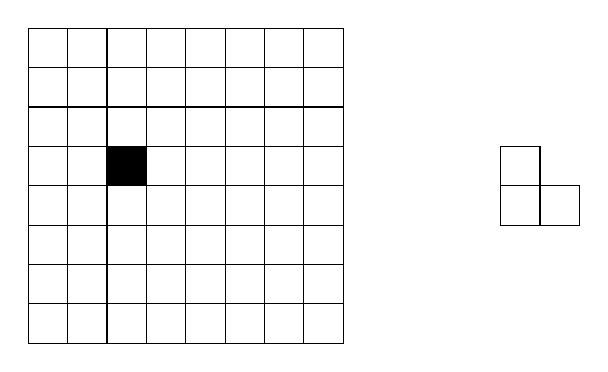
\begin{tikzpicture}[scale=0.5]
            \foreach \x in {0,1,...,7} {
                \foreach \y in {0,1,...,7} {
                    \fill[white,draw=black] (\x, \y) rectangle ++(1,1);
                }
            }
            % Fill one square with black
            \fill[black] (2, 4) rectangle ++(1,1);
            \fill[white,draw=black] (12, 3) rectangle ++(1,1);
            \fill[white,draw=black] (12, 4) rectangle ++(1,1);
            \fill[white,draw=black] (13, 3) rectangle ++(1,1);
        \end{tikzpicture}
        
        Left: an example grid with $n=3$; Right: the L-shaped tile
        
        }

        \bigskip
        
        (\emph{Hint: Use a proof by construction, i.e. design a divide-and-conquer algorithm that takes as input $n$ and $(i,j)$ with $1\leq i,j \leq 2^n$, and outputs a way to tile a $2^n\times 2^n$ grid with the black square at position $(i,j)$.}) 
        \medskip

             
    \end{tcolorbox}
    %Write your solution here!
    \section*{Solution}
    We solve the problem by designing a divide-and-conquer algorithm. The idea is to use recursion to break the \( 2^n \times 2^n \) grid into four quadrants, place one L-shaped tile at the center to “simulate” a defect in the three quadrants that do not initially contain the black square, and then recursively tile each quadrant.
    
    \bigskip
    
    \textbf{Algorithm Description:} \\
    \begin{enumerate}
        \item \textbf{Base Case:} When \( n = 1 \), the grid is \( 2 \times 2 \). Since one square is black, the remaining three squares form an L-shape, which can be covered by a single L-shaped tile.
        \item \textbf{Recursive Step:} For \( n \ge 2 \):
        \begin{enumerate}
            \item Divide the \( 2^n \times 2^n \) grid into four quadrants, each of size \( 2^{n-1} \times 2^{n-1} \).
            \item Identify the quadrant that contains the given black square (the defect).
            \item Place one L-shaped tile at the center of the grid so that it covers the central unit square of the three quadrants that do \emph{not} contain the black square. This placement introduces a new defect in each of those three quadrants.
            \item Recursively tile each quadrant:
                \begin{itemize}
                    \item In the quadrant that originally contained the black square, use that black square.
                    \item In the other three quadrants, use the square covered by the central L-tile (the newly created defect) as the black square.
                \end{itemize}
        \end{enumerate}
    \end{enumerate}
    
    \bigskip
    
    \textbf{Pseudocode:}
    
    \par\noindent\rule{\textwidth}{0.4pt}
    \smallskip        
    \textsc{TileDefectiveBoard}$(n, i, j, r, c)$ \\
    \textbf{Input:} \( n \) (the grid size is \( 2^n \times 2^n \)); \((i,j)\) is the position of the black square within the grid whose bottom-left corner is at \((r,c)\). \\
    \textbf{Output:} A tiling of the grid using L-shaped tiles.
    \begin{algorithmic}[1]
        \IF{\( n = 1 \)}
            \STATE \textbf{Place an L-tile} covering the three white squares in the \(2\times2\) grid.
            \RETURN
        \ENDIF
        \STATE Let \( m \gets 2^{n-1} \)  \COMMENT{This is the midpoint that partitions the grid}
        \STATE Determine the quadrant \( Q \) that contains the defective (black) square:
        \begin{itemize}
            \item \textbf{Quadrant 1 (bottom-left):} if \( i \le m \) and \( j \le m \).
            \item \textbf{Quadrant 2 (bottom-right):} if \( i \le m \) and \( j > m \).
            \item \textbf{Quadrant 3 (top-left):} if \( i > m \) and \( j \le m \).
            \item \textbf{Quadrant 4 (top-right):} if \( i > m \) and \( j > m \).
        \end{itemize}
        \STATE \textbf{Place one L-tile} at the center of the grid covering the central squares of the three quadrants that do not contain the original black square.
        \STATE For each quadrant \( k = 1,2,3,4 \):
        \begin{itemize}
            \item Let \((r_k, c_k)\) denote the bottom-left corner of quadrant \( k \).
            \item Let \((i_k, j_k)\) be the position of the defective square in quadrant \( k \):
            \begin{itemize}
                \item If quadrant \( k \) contains the original defective square, then \((i_k, j_k) = (i, j)\) (translated relative to the quadrant’s coordinates).
                \item Otherwise, \((i_k, j_k)\) is the position of the square covered by the central L-tile in quadrant \( k \).
            \end{itemize}
            \item \textbf{Recursively call} \textsc{TileDefectiveBoard}\((n-1, i_k, j_k, r_k, c_k)\).
        \end{itemize}
        \RETURN
    \end{algorithmic}
    \vspace{-2mm}
    \par\noindent\rule{\textwidth}{0.4pt}
    
    \bigskip
    
    \textbf{Detailed Explanation of Each Step:}
    
    \begin{enumerate}
        \item \textbf{Base Case (\( n = 1 \)):} \\
        When \( n = 1 \), the grid is a \( 2 \times 2 \) square. With one square already black, the three remaining white squares naturally form an L-shape. Thus, placing one L-tile exactly covers these three white squares.
        
        \item \textbf{Dividing the Grid:} \\
        For \( n \ge 2 \), the grid has size \( 2^n \times 2^n \). We partition the grid into four quadrants by drawing a vertical and a horizontal line through the midpoint. Each quadrant is of size \( 2^{n-1} \times 2^{n-1} \) and can be treated as an independent subproblem.
        
        \item \textbf{Identifying the Defective Quadrant:} \\
        The given black square (defect) lies in one of these four quadrants. It is crucial to identify this quadrant because it already has a defect. The other three quadrants do not have a defect, so we artificially create one in each by placing an L-tile at the center.
        
        \item \textbf{Placing the Central L-tile:} \\
        At the center of the grid, the four quadrants meet. We place one L-tile so that it covers one square in each of the three quadrants that do not contain the original defect. By doing this, each of these three quadrants now has one square covered (acting as a defect), which allows us to apply the inductive hypothesis.
        
        \item \textbf{Recursive Tiling of Each Quadrant:} \\
        Now, each quadrant is a \( 2^{n-1} \times 2^{n-1} \) grid with one defect:
        \begin{itemize}
            \item The quadrant originally containing the black square already has the defect.
            \item The other three quadrants have a new defect created by the central L-tile.
        \end{itemize}
        We then recursively apply the tiling algorithm to each quadrant. The recursion continues until the grid size reduces to \( 2 \times 2 \) (the base case).
        
        \item \textbf{Combining the Solutions:} \\
        As each quadrant is tiled recursively, the placement of the central L-tile ensures that the tilings of the four quadrants fit together perfectly. No overlaps occur, and every white square is covered by exactly one L-tile.
    \end{enumerate}
    
    \bigskip
    
    \textbf{Conclusion:} \\
    By induction on \( n \) and using this divide-and-conquer construction, we have shown that for any \( 2^n \times 2^n \) grid with one black square, the remaining white squares can be completely tiled with L-shaped tiles. This construction works regardless of the initial position of the black square, thereby proving the claim.
    
    
    
\end{document}